%Tests Results
%\begin{table}[t]                                                               
%	\caption{Torque feedback for vibration damping - Results}
%	\centering                                                                      
%	\hfill \break
%	\begin{tabular}{cc|ccc|ccc}                                                
%		\hline                                                                          
%		Velocity [mm/s] & \thead{Torque\\Feedback} & \multicolumn{3}{c|}{Arm \#xx} & \multicolumn{3}{c}{Arm \#xx2} \\ %\multirow{3}{*}{\thead{Velocity\\[mm/s]}} \thead{Torque\\Feedback} \thead{Velocity\\[mm/s]}
%		\hline
%		& & \multicolumn{6}{c}{Deviation [mm]} \\
%		& & mean & std & max & mean & std & max \\
%		\hline
%	    \multirow{2}{*}{30} & off & M & S & M & M & S & M \\
%		  & on & M & S & M & M & S & M \\
%		\hline
%			    \multirow{2}{*}{30*} & off & M & S & M & M & S & M \\
%			    & on & M & S & M & M & S & M \\
%			    \hline
%	   \multirow{2}{*}{50} & off & M & S & M & M & S & M \\
%	   & on & M & S & M & M & S & M \\
%	   \hline
%	   	   \multirow{2}{*}{50*} & off & M & S & M & M & S & M \\
%	   	   & on & M & S & M & M & S & M \\
%	   	   \hline
%	\end{tabular}
%	\label{table:results_torque}
%\end{table}

Test results are shown in table~\ref{table:results_torque}. The superscript "*" on the velocity specifies the results from the analysis on the selected regions of the trajectory showing most of the vibration. There is a significant reduction of vibration amplitude for tests performed at 50~mm/s. The presence of vibration over a biggest part of the trajectory and higher torque measurements due to the higher speed explains these results compared to trajectories performed at 30~mm/s. Moreover, no significant improvement is observed for arm PJ~00090~00009~16145~0001 at 30~mm/s. However, the maximum deviation is still reduced and contained under 1.5~mm for all tests.

Compared to the preliminary results shown in April 2016 in a presentation titled "7-DOF Arm – Vibration Investigation", smaller improvements on vibration reduction are observed from the current analysis. The major factor explaining this is the modification of the torque compensator, mainly due to stability issues. Compensator transfer function was modified to stabilize the torque loop in some configurations. Moreover, in April, the tests were performed at a constant joint speed (on joint 2 alone) instead of using a Cartesian trajectory therefore using all joints at the same time.

\begin{table}[t]
	\centering
	\caption{Torque feedback for vibration damping - Results}
	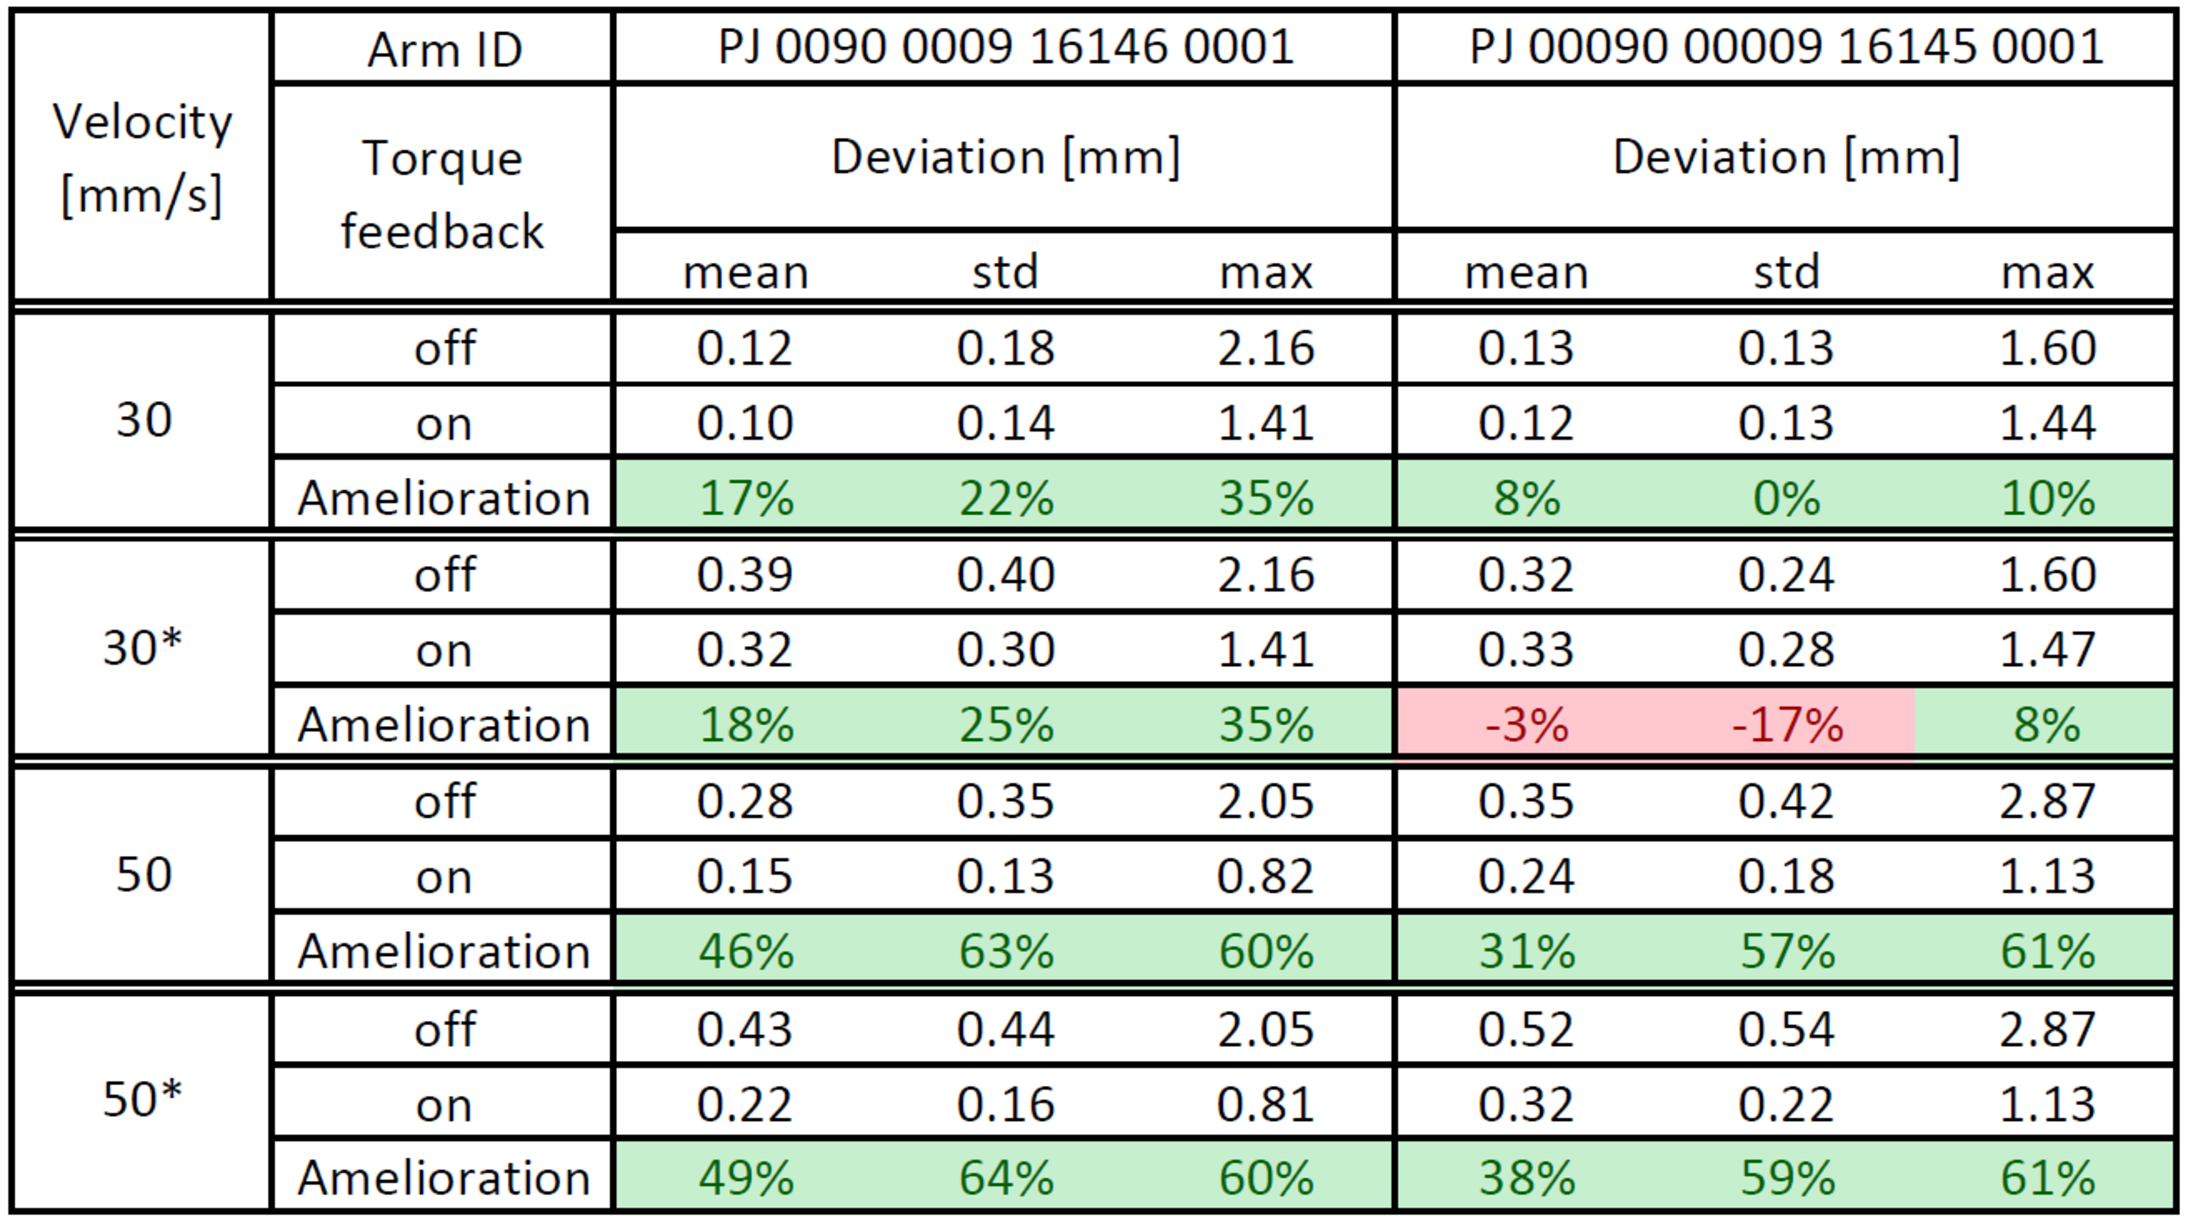
\includegraphics[width=.8\textwidth]{./images/Results.pdf}
	\label{table:results_torque}
\end{table}

To illustrate the effect of the torque feedback, the robot was hit in two direction and the following vibration was registered using the Optitrack system. The configuration of the robot and the direction of the hits are shown in fig.~\ref{fig:hitConfig}. On fig.~?? to ??, one can observe the natural frequency damping performed by the torque feedback compared to data collected when torque feedback is deactivated. 

\begin{figure}
	\begin{center}
		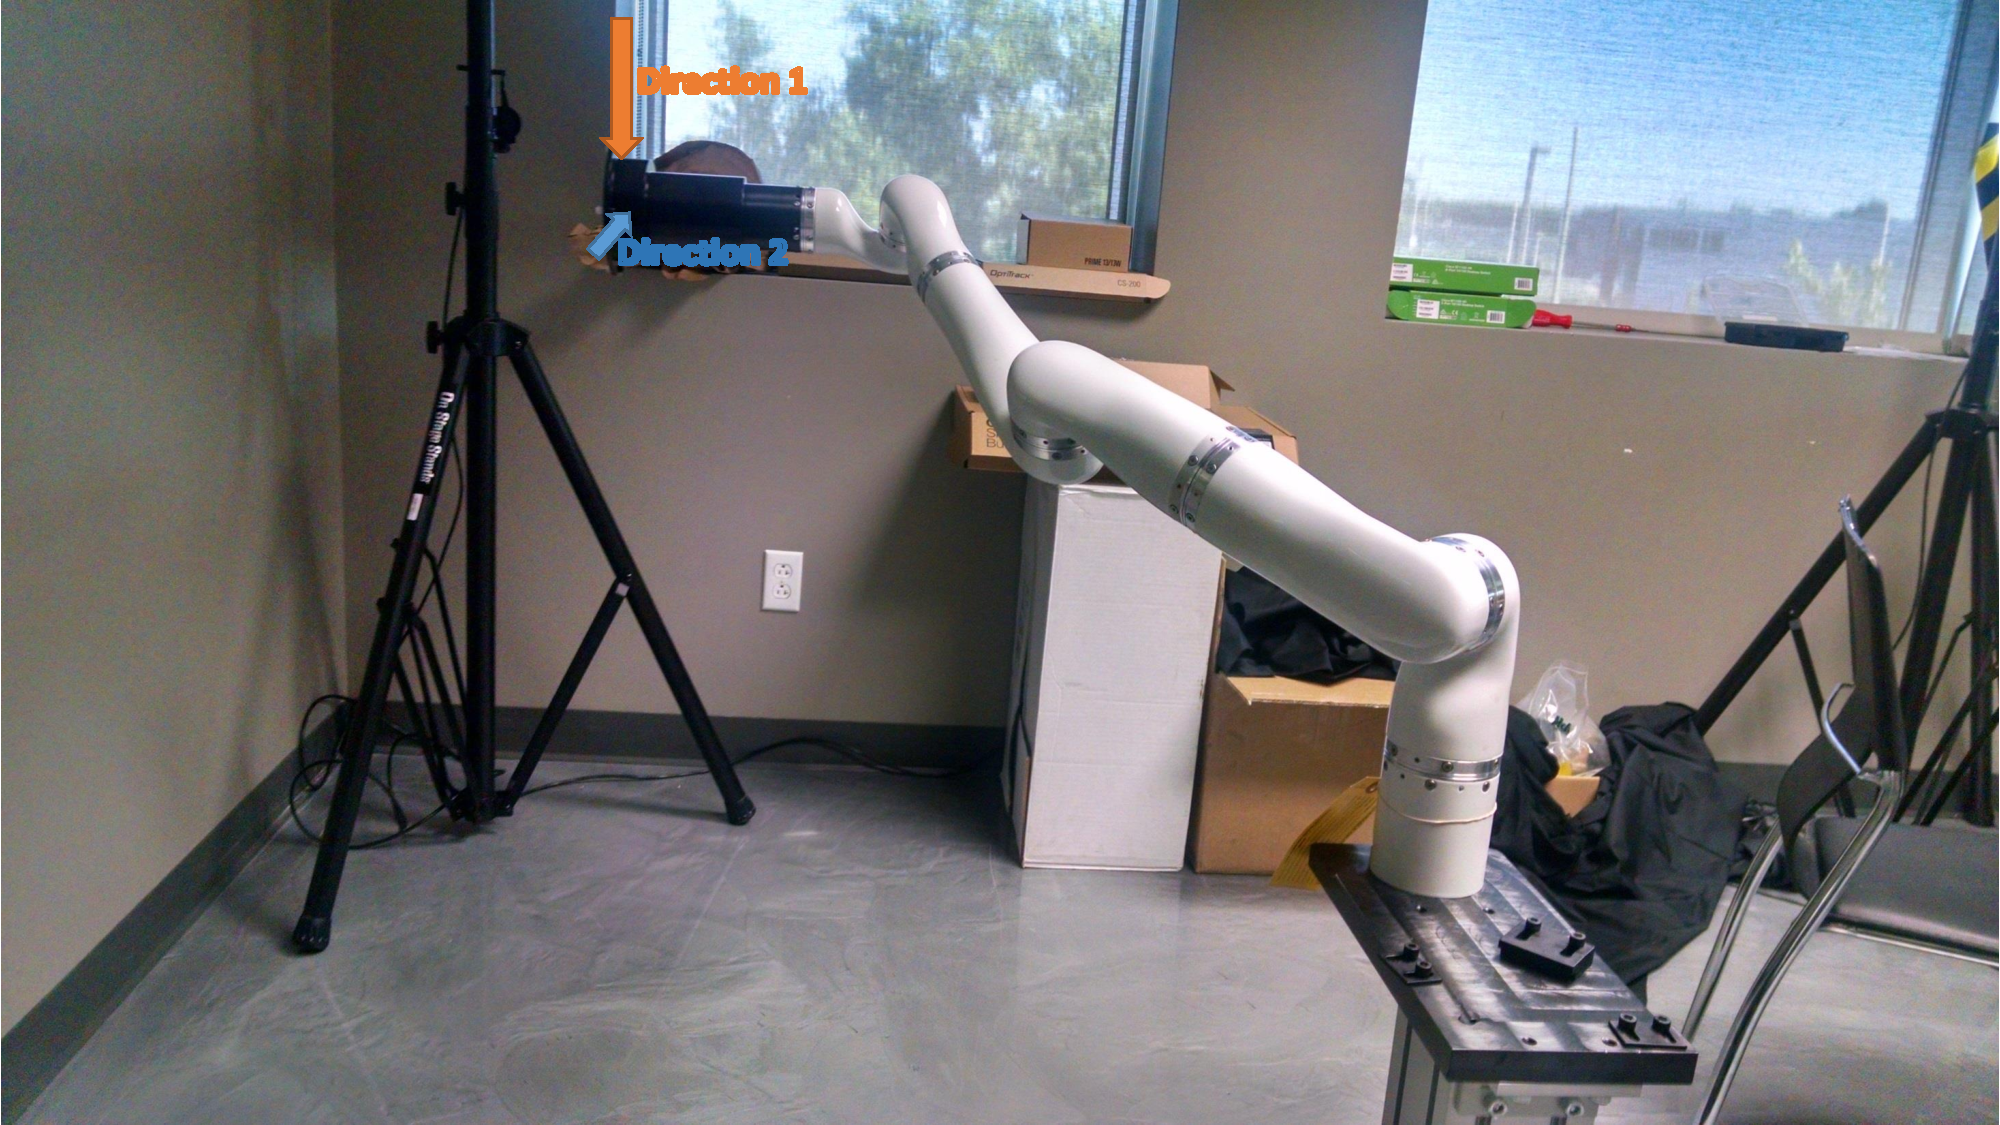
\includegraphics[width=1\textwidth]{./images/naturalVib.pdf}%
		\caption{Natural frequency damping test configuration}
		\label{fig:hitConfig}
	\end{center}
\end{figure}